% !Mode:: "TeX:UTF-8"

\externaldocument{chap2}
\externaldocument{chap3}
\externaldocument{chap4}
\externaldocument{chap5}




\chapter{智能驾驶场景下的多目标跟踪分析应用验证—— 灵动慧眼系统}

% 参考:
% /data2/whd/win10/doc/paper/doctor/doctor.Data/PDF/2687609247

%6.1  应用问题提出(多目标跟踪分析是场景理解、意图分析、预测决策的基础技术,***参考申报书***)
\section{应用问题背景}
随着国内外汽车产业的发展和城镇化的推进,智能交通技术受到世界各国政府与社会越来越广泛的重视。
2017 年 7 月,国务院颁布《新一代人工智能发展规划》~\cite{new_ai_plan},提出发展智能驾驶技术,建立智能驾驶和车路协同技术体系。
2020 年 2 月 24 日,由国家发改委、工信部、科技布等部委印发的《智能汽车创新发展战略》~\cite{car_plan_11}指出推动与人工智能、通信、互联网等行业进行深度融合,全面加速汽车产业转型。
2020 年 3 月,美国发布《智能交通系统战略规划(2020-2025)明确提出了“加速应用智能交通系统,转变社会运行方式”的愿景。
而我国人口基数大、公路网密集,由于汽车作为人们常用的交通工具,其智能化运行有着巨大的市场潜力。
同时近些年,国家“新基建”战略规划的提出和 5G 通信、人工智能等前沿技术的快速发展,为实现车对外界的信息交换(Vhicle to everything,V2X)环境下“人-车-路-云”协同的智能驾驶提供了很好的政策保证和技术支撑。
同时多目标跟踪算法作为智能驾驶实现的前提和基础,为场景理解、行为预测、意图分析等高层决策提供了强有力的支撑。
%
实现实时的多目标跟踪分析系统不仅可以提高出行的安全、运行的效率,还能加速形成具有自主知识产权的智能驾驶技术新产业集群,具有重大的经济价值和社会意义。


因此,本工作除了前面章节中多目标跟踪算法机理和技术的研究之外,也将所提出的算法在智能驾驶环境进行了工程化落地,开发出一套实时在线多目标跟踪系统——灵动慧眼。
%本项目的基本技术想定包括:智慧公共交通环境具备智能交通基础设施、智能路边单元、云中心等辅助支持,智能客车包括多传感器支持下单车智能“感知-决策-控制”技术手段,也具备V2X通信、“车-路-云”协作等技术条件。


\begin{figure*}[ht]
	\centering
	\includegraphics[width=1.0\textwidth]{figures/C6Fig/introduction.pdf}
	\caption{V2X 环境下“人-车-路-云”协同的智能驾驶跟踪感知系统示意图}
	\label{fig:introduction}
\end{figure*}


%6.2 系统需求分析   (车、路、场景的图)
% 参考:https://baijiahao.baidu.com/s?id=1708958727067894390&wfr=spider&for=pc
\section{系统需求分析}

% 系统的范围
\subsection{系统范围}
开发该系统的目的不仅仅是为了收集并保存相机采集到的实时交通场景下的画面,更是为智能驾驶场景提供支撑,对动态开放的智能驾驶场景进行实时多目标跟踪和分析,最终为行为分析、动作预测等更高层的功能提供支持。
该系统主要是一个基于视频的跟踪和分析平台,提供包括实时视频监控、目标跟踪、目标统计分析等信息。
不仅可以在线浏览和处理实时视频流信息,而且可以进行历史视频和信息的回溯。
利用“人-车-路-云”协同的方案,满足智能驾驶场景下实时感知环境的需求,成为智能驾驶场景中必不可少的模块和基础,提升交通和驾驶环境下的智能化水平。


\subsection{系统功能}
% 系统的功能(需求分析)
该系统主要的功能是为智能驾驶系统提供一套高效的感知平台,
如图~\ref{fig:introduction}所示为 V2X 环境下“人-车-路-云”协同的智能驾驶跟踪感知系统的示意图,灵动慧眼有如下几个功能:
\begin{enumerate} 
	\item \textbf{多相机支持}:可以同时配置多个 IP 相机进行同时跟踪,同时可以通过视频流来模拟 IP 相机。
	
	\item \textbf{更低的误报率}:相对于传统多目标跟踪方法,该系统使用本文所提出的多目标跟踪模型进行工程化部署,通过适量采集并标注的数据进行模型微调,并通过使用低置信度跟踪进行过滤。
	
	\item \textbf{结果显示可配置}:显示的检测结果可以进行配置选择,目前主要包括行人和车辆,但是会隐藏平均置信度,并由最常见的检测类别来确定跟踪的类别。
	
	\item \textbf{统计功能}:该系统不仅可以给出每小时的每种类别目标数的统计信息,而且记录每个计数对象交叉点详细信息,比如:相交时间、相交坐标等。	
\end{enumerate}



\subsection{性能需求}
为了实现安全高效的智能驾驶系统,需要该系统提供较高的检测、跟踪和分析的准确度,为了避免危险目标的遗漏,相比于准确率,对算法的召回率提出了更高的要求。
同时为了保证系统能够为高层功能提供实时的感知信息,该系统需要满足基本的实时性需求,实际开发和测试环境中需要达到实时的处理速度。
需要解决一系列提高运行速度的的瓶颈,包括算法性能、硬件加速、网络带宽等。

% 其他需求
%\subsection{其他需求}
%\subsection{运行环境需求}
%本系统的运行环境一般包括:

% 用户和特性
\subsection{用户和特性}
本系统根据最终所具备的功能将用户分为以下几类:
\begin{enumerate} 
	\item \textbf{算法用户}:需要为行为分析、动作预测等高层算法提供支撑;
	
	\item \textbf{监控用户}:为用户提供交通场景下实时和回放的监控画面和跟踪分析信息;
	
	\item \textbf{管理用户}:管理介入到系统中的用户和相机,保证系统的正常秩序;
	
	\item \textbf{系统管理员}:维护该系统的正常运行。
\end{enumerate}

% 系统的风险
%\subsection{系统风险}

%\subsection{安全性需求}
同时该系统在建立和运行的过程中存在一定的安全性风险:可能会产生一定的恶意用户,对建立的这个平台进行不良行为的攻击,由于该实时跟踪分析系统的有效性、实时性优于功能完备性,过多的计算请求会导致合理的跟踪分析功能不能得到实时性的满足,从而对系统的安全性产生侵害。

%\subsection{软件质量属性}




%6.3  系统架构设计   (云-边-端部署场景,软硬件平台,功能模块,功能与性能测试模块等)
\section{系统架构设计}
灵动慧眼系统的核心的实时在线多目标跟踪模块都是基于本文前面章节提出的各个模型和方法进行构建,并采用“人-车-路-云”协同的方式进行设计和部署。
该系统的检测和关联算法为第~\ref{chap:jdan} 章的联合检测关联模型,此外还以第~\ref{chap:btn}~章的类脑单目标跟踪模型作为它们的基础,
使用第~\ref{chap:nonlocal}~章和第~\ref{chap:stml}~章的基于预测的跟踪算法作为对比。
随后对前面在基准数据集上训练好的模型根据自己所采集和标注的部分视频数据进行模型微调,以增强模型的环境适应性,提高系统的跟踪和分析效果。

图~\ref{fig:system_architecture}~展示了灵动慧眼系统的架构设计。
整个多目标跟踪和分析系统主要包括三个组成模块:输入和预处理模块、云端后台处理模块、展示交互模块。
输入和预处理模块是指从各个不同的场景,包括车载摄像头、边缘端的监控摄像头、手持的智能手机摄像头等,使用 IP 相机进行数据的采集并发送到到灵动慧眼系统的流媒体服务器进行初步处理,为多目标跟踪和数据分析提供合适的输入数据。
后台处理模块是该系统最核心的部件,也是本文中各个算法及对比算法实际部署和实现的地方。
最后将跟踪和分析的结果进行页面的展示。

下面对以上每个系统子模块进行详细的介绍。

\begin{figure*}[ht]
	\centering
	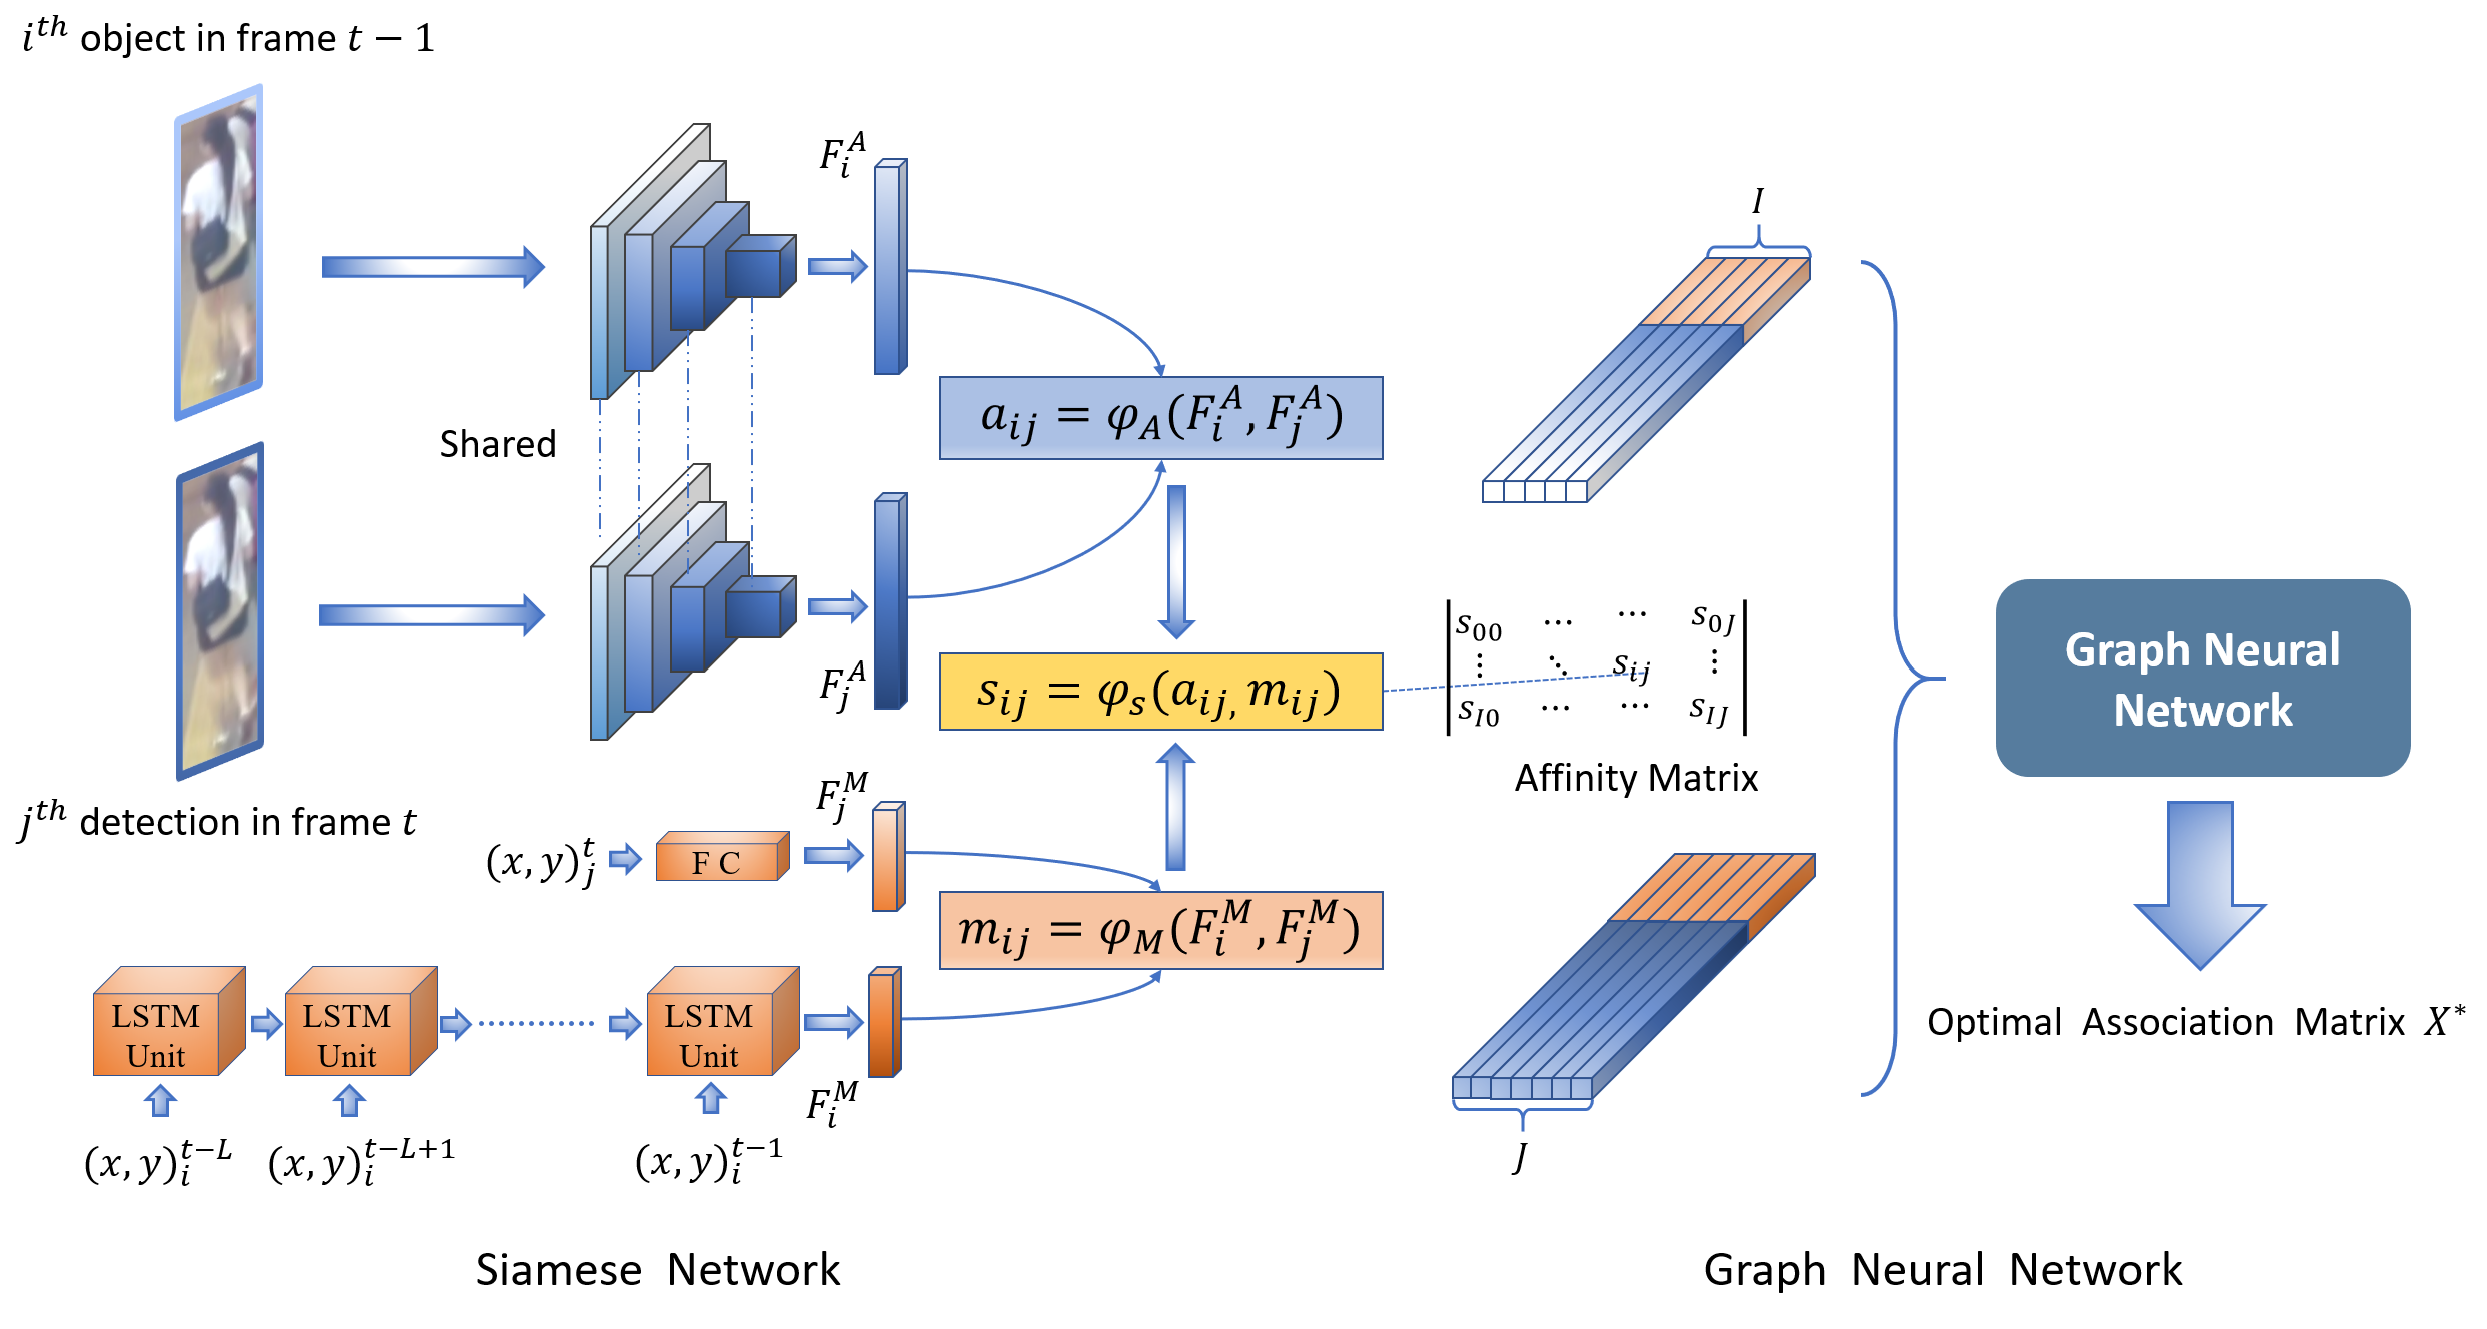
\includegraphics[width=1.0\textwidth]{figures/C6Fig/pipeline.pdf}
	\caption{灵动慧眼系统的架构设计}
	\label{fig:system_architecture}
\end{figure*}


\subsection{输入和预处理模块}
由于每个相机所处的空间位置都不同,本系统采用配置好地址和端口的 IP 相机进行输入视频信息的采集,包括智能汽车上的车载摄像头、路边边缘端安装的监控摄像头、行人手持的移动智能手机摄像头等设备,并将不同数据源的视频流数据同时进行处理。
每个车载端或者边缘端的相机都作为一个实时视频数据源服务,通过 RTSP 协议,利用有线或者无线网络实时地向流媒体服务端发送视频流数据。
为了解决流媒体服务器或云端后台处理模块来不及处理视频流数据,导致视频帧堆积的问题,该系统在预处理模块采用生产者消费者模式,建立一个作为临时缓存的生产队列,队列中保存从车载端和边缘端发送过来的视频帧数据。
然后启动一个消费者线程读取生产队列前端中的最新视频帧数据,这样保证后续模块每次处理的都是最新的一帧。
同时将接收到的所有视频数据都保存到数据库服务器中进行备份,以便用户可以通过信息回放功能查看历史视频数据。
服务器端再通过应用程序路由转发给响应的后台处理模块响应的函数进行视频数据的处理,并将最新的视频帧缩放成检测跟踪模型输入所需要的尺寸。


\subsection{云端后台处理模块}
图~\ref{fig:system_architecture} 中的云端后台处理模块简要说明了灵动慧眼系统的实时在线多目标跟踪过程。
对数据传输和预处理模块传输过来的输入图像帧预测其中所有目标的当前目标表征。
然后使用第~\ref{chap:jdan} 章的联合检测关联模型,将当前目标表征和历史表征传递到连接子模块和关联子模块以生成对应的关联矩阵,并通过匹配算法将结果更新到跟踪轨迹管理器中。
跟踪轨迹管理器中存储的历史帧的跟踪信息,以及历史轨迹与当前帧中检测到的目标的相似度之和。
在云端后台处理模块中一个跟踪轨迹对应于一个被跟踪目标的实体。
当接收到一个新的目标表征后,跟踪轨迹管理器将保留表征并将所有历史表征输出到关联子模块以生成每个历史帧和当前帧之间的关联矩阵。
之后更新跟踪轨迹管理器,并生成当前帧中的跟踪结果,传递给展示交互模块。
同时在跟踪过程中将原始视频和所产生的跟踪和以及分析统计信息保存到数据库服务器,用于后面对历史信息进行回放和查询。

该模块使用的联合检测关联模型属于一阶段的端到端在线多目标跟踪模型,其中每个被跟踪目标的外观特征在整个系统的处理流程中只提取了一次,同时将提取到的外观特征保存下来供将来的关联步骤使用。
为了提高系统的响应速度,在测试和部署时使用高性能的计算机硬件进行加速,特别是使用计算能力强的显卡优化联合检测关联模块的计算过程,使灵动慧眼系统能在实际运行中基本达到工程化的实时性要求。
这对于智能驾驶系统的及时感知和预测有着至关重要的作用,提升了系统的实时性和安全性。

为了保证该系统对其他检测跟踪算法的可扩展性,可以使用其他检测跟踪算法替换本文所提出的方法,以便进行不同算法的测试和对比,实现系统模块内的高内聚和模块间的低耦合。
主要可以替换和测试一些经典的检测跟踪算法和最新的且精度较高的算法,测试不同算法在不同驾驶场景下的跟踪和分析效果,便于找出算法的不足之处以便进行优化和改进。



\subsection{展示交互模块}
由于根据函数路由返回的流式响应视频流需要在网页中显示,所以展示交互模块使用客户端浏览器显示跟踪和分析结果的视频流来自动更新页面中的图像元素。
可以使用不同的客户端,比如 PC 终端、智能手机等从 Web 服务器获取跟踪和统计分析信息并进行实时地显示。
在该系统中,对于每个检测并跟踪到的目标都会对当前目标的总计数进行记录的更新。
当相机视野中出现一个新的类别,即每检测到一个新的类别还会创建一个新的类计数器。
灵动慧眼系统除了跟踪和分析常见的行人,还可以通过配置进行比如行人、车辆等多个类别的多目标跟踪和统计分析。
使该系统能很好地对变化中的需求进行适应,以达到更好的应用效果,对高层应用和用户使用提供了更高的支撑。

该模块仅仅用于用户与系统的展示和交互上,对于多目标跟踪的过程和为其场景分析功能的添加只起到调试和显示效果,在真实工程化部署时可以进行配置并省略,以减少系统的开销,提高系统的运行速度和增强实时响应能力。


\subsection{系统部署和性能评测}
灵动慧眼系统的运行环境包括操作系统及其版本,服务器端采用 Ubuntu 18.04 及以上版本,客户端可以为任意的 PC 终端、手机移动端等;
系统数据传输和预处理模块的输入端基于 RTSP 实时流协议使用 IP 相机收集车载端、边缘端以及其他视频数据,并向流媒体服务端发送视频流数据。
服务器端的云端后台处理模块使用 OpenCV、TensorFlow~\cite{abadi2016tensorflow}、Pytorch~\cite{paszke2019pytorch} 等 Python 库进行实现。
整个云端后台处理模块部署在 128G 内存的 20 核且拥有 4 块 RTX 2080 GPU 的高性能服务器上,可以为其他更高级的场景分析和用户浏览提供实时服务。
目前主要的跟踪服务主要运行在云端,并测试多路相机输入时的跟踪情况。
系统展示交互模块的网页前端~\footnote{https://flask.palletsprojects.com/en/2.0.x/}及服务端使用轻量级的 Flask~\footnote{https://github.com/LeonLok/Multi-Camera-Live-Object-Tracking} 框架进行实现。


将高分辨率的单个摄像机流在以 30 FPS 的速度进行流式传输时,在服务器上托管下平均可提供约 15 FPS 的检测跟踪速度。
由于该系统支持多个车载端和边缘端的 IP 相机进行视频流输入,但是服务器资源有限,同时处理多个视频流将会一定程度上降低多目标检测跟踪和分析的速度。
降低处理视频流的分辨率或图像质量将提高系统的运行速度,但同时也会降低检测跟踪的精度。
在基本满足实时性的要求时,需要在速度和精度之间做出权衡,以获得最佳的系统效果。
同时还有很多其他因素会影响灵动慧眼系统的整体性能,比如网络信道质量、带宽等。




%6.4  系统测试 (按照功能、性能指标,分场景(目标密集、目标稀疏;高速、低速;场景清晰,场景复杂等),多个对比算法)
\section{系统测试和验证}
为了说明该系统的有效性,分别从定量和定性两个角度展示灵动慧眼系统的实际效果。
首先进行定量化测试和验证,将本文的方法和一些经典多目标跟踪算法在同样的智能交通场景视频进行多目标跟踪并把结果保存下来,并利用手工标注的方法获得跟踪所对应的真实值,然后如图~\ref{tab:quantitative_test} 所示计算出多目标跟踪性能评价指标,可以看出本文所提出的方法在智能驾驶场景下有较大的优势。

\vspace{0.5em}
\renewcommand\arraystretch{1.5}
\begin{figure}[htbp]
	\centering
	
	\subfigure[动态开放交通场景下车辆的跟踪和统计效果]{
		\begin{minipage}[t]{0.90\linewidth}
			\centering
			\includegraphics[width=1\textwidth]{figures/C6Fig/cidi_car.pdf}
		\end{minipage}%
	}%
	%	\subfigure[With STURE]{
		%		\begin{minipage}[t]{0.48\linewidth}
			%			\centering
			%			\includegraphics[width=1\textwidth]{figures/C6Fig/dongfanghong.pdf}
			%		\end{minipage}%
		%	}%
	
	\subfigure[动态开放场景下行人的跟踪和统计效果]{
		\begin{minipage}[t]{0.90\linewidth}
			\centering
			\includegraphics[width=1\textwidth]{figures/C6Fig/cidi_person.pdf}
		\end{minipage}
	}%
	%	\subfigure[Tracking results with STURE]{
		%		\begin{minipage}[t]{0.48\linewidth}
			%			\centering
			%			\includegraphics[width=1\textwidth]{figures/C6Fig/experiment.pdf}
			%		\end{minipage}
		%	}%
	
	\centering
	\caption{灵动慧眼系统多相机多类型跟踪统计效果展示}
	\label{fig:system_present}
\end{figure}

\vspace{0.5em}
\renewcommand\arraystretch{1.5}
\begin{table}[htbp]\wuhao
	\centering
	\caption{智能驾驶场景下不同方法之间性能的比较}
	\vspace{0.3em}
	%\vspace{0.5em}\wuhao{\textwidth}
	\begin{tabular}{c|cccccccccc}
%		\hline
		\hline
		方法   & MOTA$ \uparrow $ & MOTP$ \uparrow $  & IDF1$ \uparrow $  & IDR$ \uparrow $ & FP$ \downarrow $  & FN$ \downarrow $  & MT$ \uparrow $  & ML$ \downarrow $  & IDS$ \downarrow $  & Frag$ \downarrow $\\ 
		%		\midrule[1.0pt]
		\hline
		PHD\_DAL~\cite{2019Online}    &36.9 &68.1 &29.5 &37.2 &150 &452 &6.5 &53.7 &375 &438\\
		HISP~\citep{baisa2021robust}   &37.2 &70.8 &30.1 &39.5 &150 &366 &8.7 &43.1 &247 &347\\
		GMPHD\_ReId~\citep{baisa2021occlusion}  &37.3 &73.3 &41.2 &30.8 &114 &252 &8.6 &42.8 &165 &157\\
		DASOT17~\citep{chu2020dasot}   &40.1 &71.1 &36.2 &27.9 &217 &363 &8.2 &39.3 &121 &240\\
		NAAL   &45.2 &\bfseries73.8 &\bfseries50.1 &40.9 &151 &215 &9.2 &41.3 &92 &107\\
		STURE     &47.1 &73.2 &48.2 &34.6 &\bfseries51 &\bfseries123 &\bfseries11.2 &41.0 &73 &35\\
		JDAN     &\bfseries53.7 &73.5 &41.2 &\bfseries47.2 &143 &493 &9.16 &\bfseries36.8  &\bfseries31 &\bfseries24\\
		\hline
%		\hline
		%		\bottomrule[1.5pt]		
	\end{tabular}
	\label{tab:quantitative_test}
\end{table}

如图~\ref{fig:system_present} 所示按照功能、场景、算法等方面展示系统验证的效果。
选取了两个典型的实时场景进行多目标跟踪和统计的功能验证效果展示,其中图~\ref{fig:system_present}(a) 展示了动态开放十字路口的多目标车辆跟踪和统计的效果,图~\ref{fig:system_present}(b)展示了典型室外场景下的多目标行人跟踪和统计的效果,表明该系统在典型动态开放场景下能实现同时进行不同类型目标的跟踪和分析,很好地实现了该系统的功能需求。


\vspace{0.5em}
\renewcommand\arraystretch{1.5}
\begin{figure*}[ht]
	\centering
	\includegraphics[width=0.8\textwidth]{figures/C6Fig/system_test.pdf}
	\caption{灵动慧眼系统在具有挑战性的环境下的测试}
	\label{fig:system_test}
\end{figure*}

% Faster RCNN~\cite{b8} 和 YOLOv3~\cite{redmon2018yolov3}
图~\ref{fig:system_test} 中显示了该系统在具有各种挑战条件下进行响应的验证,选取了阴天或者雨天等光照不足的天气情况作为基本背景,以测试该跟踪分析系统应对复杂极端情况的能力。
图中第一行的两图分别表示在目标稠密和稀疏的交通场景下系统的运行效果,第二行分别表示智能汽车在高速和低速运动时的跟踪和分析结果,第三行表示使用其他方法进行测试时的效果,这里使用经典的 PHD\_DAL~\cite{2019Online} 和 DASOT17~\citep{chu2020dasot} 作为测试对比方法,这种情况下存在一定的检测和跟踪错误,反过来证明本文所提出的方法在应对有挑战的现实环境下具有较强的鲁棒性。

以上测试和验证效果均表明该系统在现实动态开放场景下能取得不错的性能并产生较大的实际应用价值。



%6.5  本章小结(应用效果,如何服务于其他模块;验证前面算法效果;从应用的角度强调内脑计算分析的有点)
\section{本章小结}
基于本文研究工作所开发的灵动慧眼系统,实现 V2X 智能驾驶环境下“人-车-路-云”的协同感知,不仅能够自动进行目标的检测和跟踪,还能提供所关注环境中的统计信息,如目标交汇、速度、方向等,同时在实际测试过程中表现出较好的效果和实时性。
该系统不仅仅提供自动实时地监控服务,极大地减少了人力消耗,同时为人和其他算法进行高层次的分析和决策提供助力,增强驾驶场景下的智能化水平,帮助智慧城市的实现。
该系统以人工智能作为促进社会智能化发展的新手段,为社会的文明和进步做出贡献。




